
\section{はじめに}
屋内位置置推定技術は,現代社会において重要な役割を果たしており様々な活用が期待できる.
屋内位置推定技術が使用される一例として,ショッピングモール施設でのナビゲーションシステムが挙げられる[1].
このシステムでは顧客が店内で商品を探している際,その位置情報を元にしたナビゲーションシステムを通じて目的の商品が置かれている売り場まで案内するシステムである.

屋外における位置推定技術としてGPSが広く利用されているが,屋内環境では建物の壁や天井がGPS衛星からの電波を遮断してしまい,位置推定精度が大きく低下してしまう問題があり,別のアプローチが必要とされている.
屋内位置推定手法として,PDR(Pedestrian Dead Reckoning)が挙げられる.
PDRは主に,加速度計,ジャイロスコープ,磁気センサなどのセンサを利用して歩行者のステップ数,歩行速度,歩行方向を推定する.
その情報を元に歩行者がどのくらいの距離をどの方向に移動したかを累積的に計算して基準となる位置からの相対的な位置を推定する手法である.
他の例として,Wi-Fiの電波を使用した屋内位置推定手法がある.
Wi-Fiを利用した屋内位置推定は,Wi-Fiアクセスポイントからの信号強度を利用して位置推定を行う.特定の地点でのフィンガープリントを予め取得しておきそれと比較して推定を行う手法や,3つのアクセスポイントからの電波強度を利用して三角測量を行う手法がなどがある.

しかしこれらの手法は特定の状況や環境に特化したものであり,すべての屋内環境で同様の効果を発揮するわけではない.例として先ほどあげたWi-Fiを利用した屋内位置推定の場合,地下施設やWi-Fiアクセスポイントが設置が難しい場所では,信号が弱いため正確な位置推定が難しくなる.
PDRの場合各種センサによる誤差が蓄積されるため,時間経過とともに誤差が大きくなってしまう問題がある.そのため長時間の屋内移動場合は精度が低下してしまう.

これらの問題を解決するためには状況や環境に応じて適切な位置推定手法の選択または組みわせる必要がある.
本研究の目的は様々な環境に対応できるオフライン屋内位置推定ライブラリの検討である.
ここでいうオフラインとは,あらかじめ取得したデータを元に位置推定を行うという意味である.
先ほどあげた長時間の屋内移動の場合,PDRで推定した位置情報をWi-Fiの電波強度を利用した位置推定でセンサの誤差を修正すれば,より正解な位置推定を行える.
これらの補正を自由に組み合わせて使えるライブラリの検討を行い,様々な状況に対応できるオフライン屋内位置推定ライブラリを実現する.

\begin{figure}[h]
	\centering
	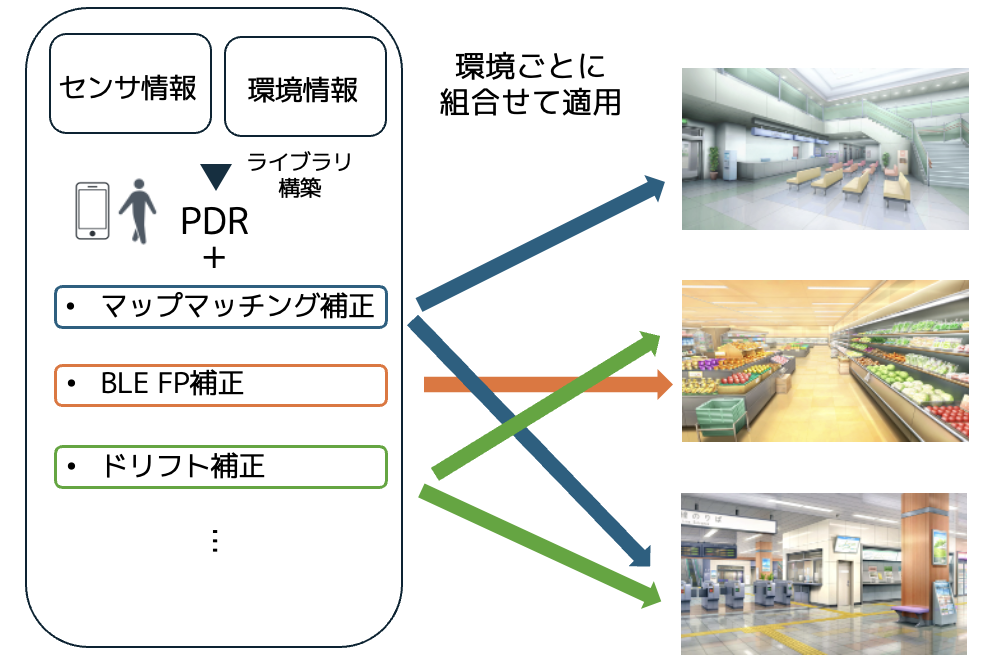
\includegraphics[width=80mm]{image/first.png}
	\caption{様々な状況と環境に対応できる\\PDRベースの
		屋内位置推定ライブラリの概要}    \label{fig:gt-trajectory}
\end{figure}
